Our aim in this experiment is to measure superconductor to normal tunneling as described above. To achieve this we choose Aluminum as the superconductor and Lead as the normal conductor. This is convenient because $Pb$ and $Al$ have different transition temperatures of $1.140 K$ and $7.193 K$ respectively. Therefore the range in between the two allows the observation of the desired effect. Another benefit is that Aluminum readily oxidizes to $Al_2O_3$ at room temperature, providing an insulating layer.

\subsection{Sample Preparation}
Sample preparation was done in a manner similar to the one described in \cite{giaever2}. First a thin layer of Aluminum was vapor-deposited by means of a heated spiral filament onto a microscope slide in a vacuum chamber. Air was then let into the chamber, allowing a thin insulating film of $Al_2O_3$ to form. Finally the chamber was evacuated again, and the last layer, consisting of $Pb$, was deposited.

\begin{figure}[h!]
\centering
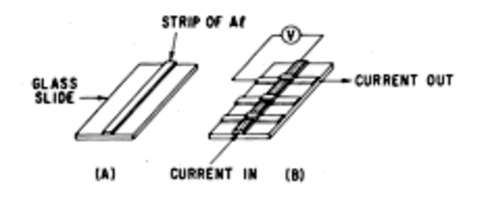
\includegraphics[width=0.4\textwidth]{sample.pdf}
\caption{Slide layout\label{sample}}
\end{figure}

The layers were deposited in the shape of strips, a long strip of $Al$ crossed by 5 shorter strips of $Pb$, providing up to 5 tunnel junctions per slide. A similar arrangement can be seen in fig. \ref{sample}. The shapes of the layers were determined by placing a mask between the heated filament and the slide.

To estimate the thickness $h$ of the films  we assumed an isotropic distribution of the evaporated metal and measured the distance $r$ between heating spiral and slide, giving us 
\begin{equation}\label{thickness1}
h=\frac{V}{4\pi r},
\end{equation}
with $V$ the volume of the metal piece to be evaporated.

We also tried to measure the thickness indirectly via the resistance $R$ of the strips, knowing their width $b$ and length $l$. According to Ohms law 
\begin{equation}\label{thickness2}
h=\frac{\rho l}{Rb}. 
\end{equation}

However, the films are so thin that the random distribution of the particles and possibly also percolation effects prevent this method from being useful. The layer thickness estimated by the first method was of the order of $100nm$, whereas with the second it was $10nm$, a difference factor of $10$.

With a thickness of some nanometers the deposited metal atoms form valleys and hills, distinguishable enough not to ignore them. The measured resistance corresponds to the minimum thickness the current finds in its way, i.e. the maximum resistance. Therefore the thickness estimated with equation \eqref{thickness2} gives a too small value compared with the average.

The thickness of the insulating layer, and thus the Normal-Normal resistivity of the sample was controlled by varying the time the sample was left at the air. We tried several periods of time, with the final sample being prepared with 10 minutes (time from opening the valve to restarting of the vacuum pump).

There are two main reasons for preparing the samples in a vacuum. Firstly it is necessary to keep the layers as free from contamination as possible, because due to their thinness even small amounts of foreign substances might cause a change in behavior. Secondly the vacuum significantly reduces scattering effects, making the thickness of the deposited layers as homogenous as possible. This is necessary so that the current is distributed evenly across the junction.

We used an oil diffusion pump to attain a high vacuum of about $10^{-6}\text{torr}$.

\subsection{Measurement}
The sample was immersed in a cryostat containing liquid $He$ surrounded by a layer of liquid $N$. A rotary pump was connected to the cryostat to reduce pressure inside. Since the vapor pressure is linked to the temperature of the Helium this allowed us to perform measurements at several temperatures. A mechanical manometer was also connected to the chamber.

\begin{figure}
\centering
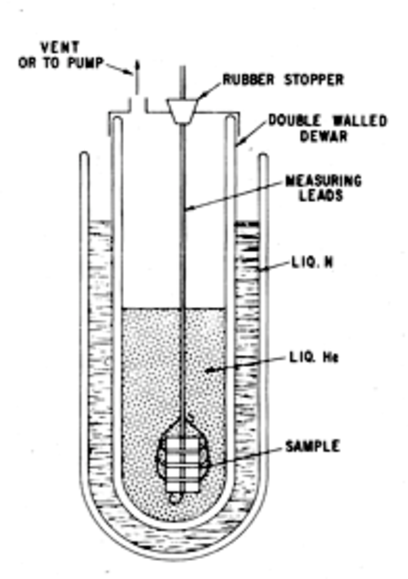
\includegraphics[width=0.35\textwidth]{cryostat.pdf}
\caption{Cryostat layout\label{cryostat}}
\end{figure}

%MYSTERY: $p_{bottom} = p_{top}$?\\

The tunnel junction was connected in a 4 terminal configuration, i.e. the voltage and current were measured in two separate circuits, which only joined at the tunneling junction. This setup has the advantage that only the potential difference at the junction itself is measured, and factors such as the resistivity of cables leading up to the sample, and the change with temperature thereof, do not have to be taken into account. 

In our setup the Ampere-meter also functioned as a current source. Both units were connected to a computer via an IEEE interface, which was used to set the current and record the readings. In each measurement run, the voltage across the junction was measured for a range of equally spaced current intensities, as produced by said current source.  We measured ranges from $50 \mu A$ to $5 mA$ using divisions between 100 and 2000 steps. A time of $1s$ was left between measurements to allow for the readings to stabilize.

The resolution of voltage measurements depended greatly on the range in which the measurement was taken. The Volt-meter automatically changes the resolution, therefor we tried to avoid such changes of resolution by setting corresponding limits on the current. When the data contained a change of scale we omitted the data points beyond the change. The effects of this change of resolution are most severe in the numerical derivation, since this is done by dividing the differences.


